\documentclass[twoside]{article}
\usepackage{format/aistats2e}
\usepackage{amssymb,amsmath,amsthm}
\usepackage{graphicx}
\usepackage{preamble}
\usepackage{natbib}
\usepackage{hyperref}
\usepackage{color}
\definecolor{mydarkblue}{rgb}{0,0.08,0.45}
\hypersetup{ %
    pdftitle={},
    pdfauthor={},
    pdfsubject={},
    pdfkeywords={},
    pdfborder=0 0 0,
    pdfpagemode=UseNone,
    colorlinks=true,
    linkcolor=mydarkblue,
    citecolor=mydarkblue,
    filecolor=mydarkblue,
    urlcolor=mydarkblue,
    pdfview=FitH}
    
    
% If your paper is accepted, change the options for the package
% aistats2e as follows:
%
%\usepackage[accepted]{aistats2e}
%
% This option will print headings for the title of your paper and
% headings for the authors names, plus a copyright note at the end of
% the first column of the first page.


\begin{document}

% If your paper is accepted and the title of your paper is very long,
% the style will print as headings an error message. Use the following
% command to supply a shorter title of your paper so that it can be
% used as headings.
%
%\runningtitle{I use this title instead because the last one was very long}

% If your paper is accepted and the number of authors is large, the
% style will print as headings an error message. Use the following
% command to supply a shorter version of the authors names so that
% they can be used as headings (for example, use only the surnames)
%
%\runningauthor{Surname 1, Surname 2, Surname 3, ...., Surname n}

\twocolumn[

\aistatstitle{Kernel Structure Discovery in Gaussian Process Models}

\aistatsauthor{ Anonymous Author 1 \And Anonymous Author 2 \And Anonymous Author 3 }

\aistatsaddress{ Unknown Institution 1 \And Unknown Institution 2 \And Unknown Institution 3 } ]

\begin{abstract}
Gaussian process (GP) models are used widely and successfully.  However, their effictiveness depends critically on choosing an appropriate family of kernels.  This aspect of GP modeling has been sorely underdeveloped.  In this paper, we introduce a procedure for automatically and efficiently searching through a large space of GP models.
\end{abstract}

\section{INTRODUCTION}

Similar searches over large model classes have been succesfully used in machine vision [cite Cox + Pinto].  In general, learning the model class from data seems superior proposing the model beforehand.  In high dimensional problems, it is also hard for a practitioner to propose an appropriate model even after examining a dataset closely.  Choosing a kernel family is also a stumbling block for non-experts who wish to use Gaussian Process models.

\section{GP STRUCTURE}

[Standard GP intro \cite{rasmussen38gaussian}]

\section{MODEL-BASED SEARCH OVER MODELS}

Bayesian optimization for hyper-parameter search: \cite{snoek2012practical}

\subsection{Bayesian Optimization}

cite Ryan Adams, Lizotte, de Frietas

\subsection{A Kernel between kernels}

Hyperkernels \cite{ong2002hyperkernels}


\section{RELATED WORK}

Compositional Model search for unsupervsied learning: \cite{grosse2012exploiting}



Hyperkernels \cite{ong2002hyperkernels}

\subsection{ANOVA Kernels}

Additive Gaussian Processes \cite{duvenaud2011additive11}

Support vector regression with ANOVA decomposition kernels \cite{stitson1999support}

\subsubsection{Smoothing spline ANOVA models}

A closely related procedure from the statistics literature is smoothing-splines ANOVA (SS-ANOVA)\cite{wahba1990spline, gu2002smoothing}. An SS-ANOVA model is estimated as a weighted sum of splines along each dimension, plus a sum of splines over all pairs of dimensions, all triplets, etc, with each individual interaction term having a separate weighting parameter.  Because the number of terms to consider grows exponentially in the order, in practice, only terms of first and second order are usually considered.  Learning in SS-ANOVA is usually done via penalized-maximum likelihood with a fixed sparsity hyperparameter.

\subsection{Hierarchical Kernel Learning}

In "High-Dimensional Non-Linear Variable Selection through Hierarchical Kernel Learning", Bach\cite{DBLP:journals/corr/abs-0909-0844} uses a regularized optimization framework to learn a weighted sum over an exponential number of kernels which can be computed in polynomial time.  The subsets of kernels considered by this method are restricted to be a \textit{hull} of kernels.\footnote{In the setting we are considering in this paper, a hull can be defined as a subset of all terms such that if term $\prod_{j \in J} k_j(\bf x, x')$ is included in the subset, then so are all terms $\prod_{j \in J / i} k_j(\bf x, x')$, for all $i \in J$.  For details, see \cite{DBLP:journals/corr/abs-0909-0844}.}
Given each dimension's kernel, and a pre-defined weighting over all terms, HKL performs model selection by searching over hulls of interaction terms.
% \subsubsection{All-subsets kernel with uniform weightings}
In \cite{DBLP:journals/corr/abs-0909-0844}, Bach also fixes the relative weighting between orders of interaction with a single term $\alpha$, computing the sum over all orders by:
\begin{equation}
\label{eqn:uniform}
k_{a}({\bf x, x'}) = v_D^2 \prod_{d=1}^D \left(1 + \alpha k_{d}(x_{d}, x_{d}') \right)
\end{equation}
which has computational complexity $O(D)$.  However, this formulation forces the weight of all $n$th order terms to be weighted by $\alpha^n$.

The main difficulty with the approach of \cite{DBLP:journals/corr/abs-0909-0844} is that hyperparameters are hard to set other than by cross-validation.  In contrast, our method optimizes the hyperparameters of each dimension's base kernel, as well as the relative weighting of each order of interaction. 

Accuracy versus interpretability in flexible modeling: Implementing a tradeoff using Gaussian process models \cite{plate1999accuracy}

A related functional ANOVA GP model\cite{kaufman2010bayesian} decomposes the \emph{mean} function into a weighted sum of GPs. However, the effect of a particular degree of interaction cannot be quantified by that approach. Also, computationally, the Gibbs sampling approach used in \cite{kaufman2010bayesian} is disadvantageous.

\subsection{Genetic Searches}

Evolving kernel functions for SVMs by genetic programming: \cite{diosan2007evolving}

A Genetic Programming based kernel construction and optimization method for Relevance Vector Machines: \cite{bing2010gp}

\subsection{Equation Learning}

Equation discovery with ecological applications \cite{dzeroski1999equation}

Discovering admissible model equations from observed data based on scale-types and identity constraints \cite{washio1999discovering}

\subsection{Multiple Kernel Learning}

Christoudias et al.\cite{christoudias2009bayesian} previously showed how mixtures of kernels can be learnt by gradient descent in the Gaussian process framework.  They call this \emph{Bayesian localized multiple kernel learning}.


\section{EXPERIMENTS}

\subsection{Real datasets}

\subsubsection{Maunal Loa Atmoshperic Carbon Dioxide}

As an example of a GP modeling problem where choosing an appropriate structure is critical, we revisit a dataset explored in \cite{rasmussen38gaussian}, pages 120-126, where a kernel was hand-tailored to fit a GP model to the dataset.

\begin{figure}
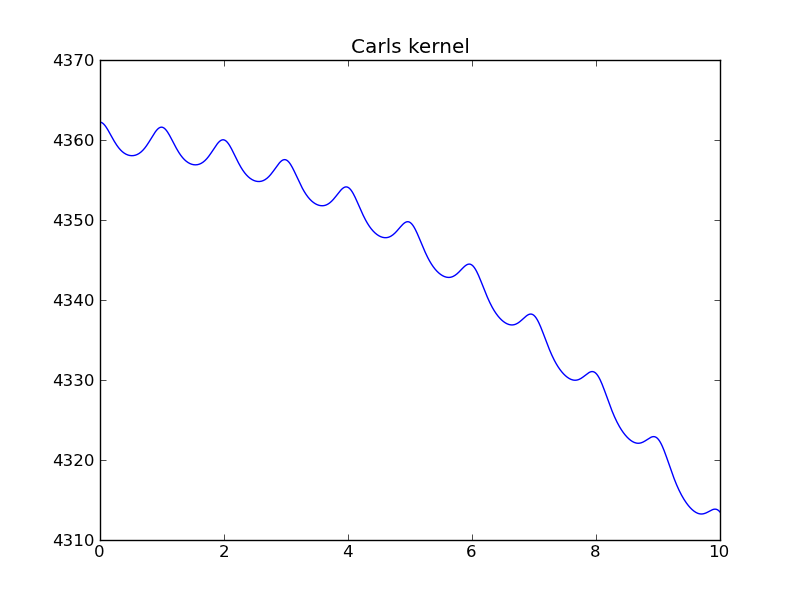
\includegraphics[width=\columnwidth]{../figures/carls_kernel}
\caption{Carl's kernel function on the Mauna dataset.}
\end{figure}

\begin{figure}
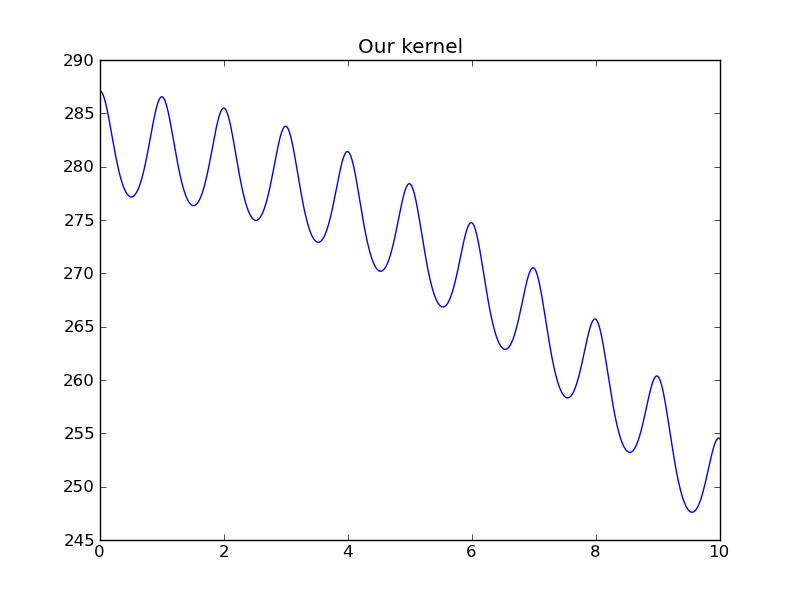
\includegraphics[width=\columnwidth]{../figures/our_kernel}
\caption{Our best kernel function on the Mauna dataset.}
\end{figure}

\begin{figure}[h]
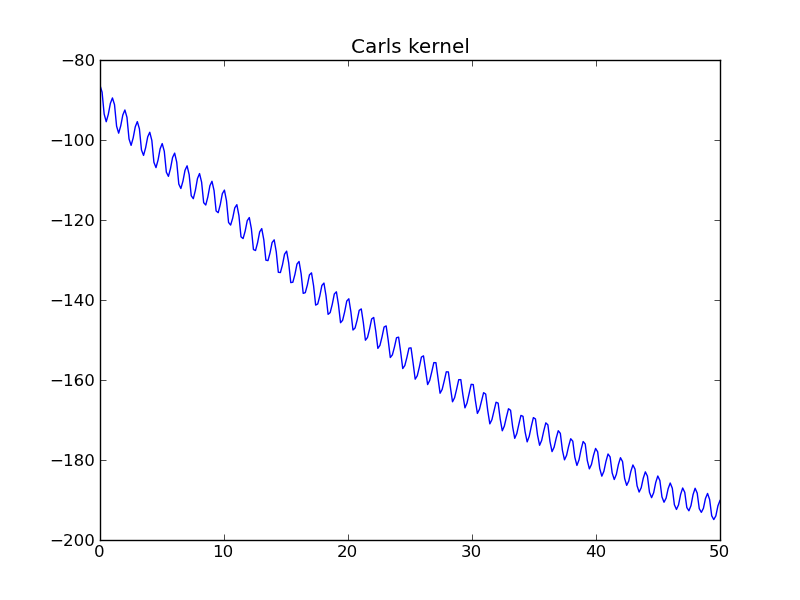
\includegraphics[width=\columnwidth]{../figures/carls_kernel_draw1}
\caption{A draw from Carl's kernel.}
\end{figure}

\begin{figure}[h]
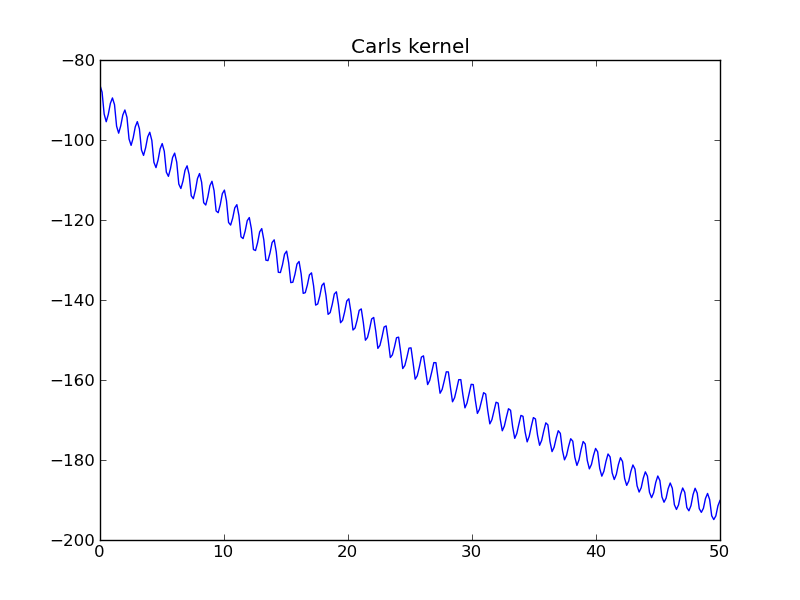
\includegraphics[width=\columnwidth]{../figures/carls_kernel_draw1}
\caption{Another draw from Carl's kernel.}
\end{figure}

\begin{figure}[h]
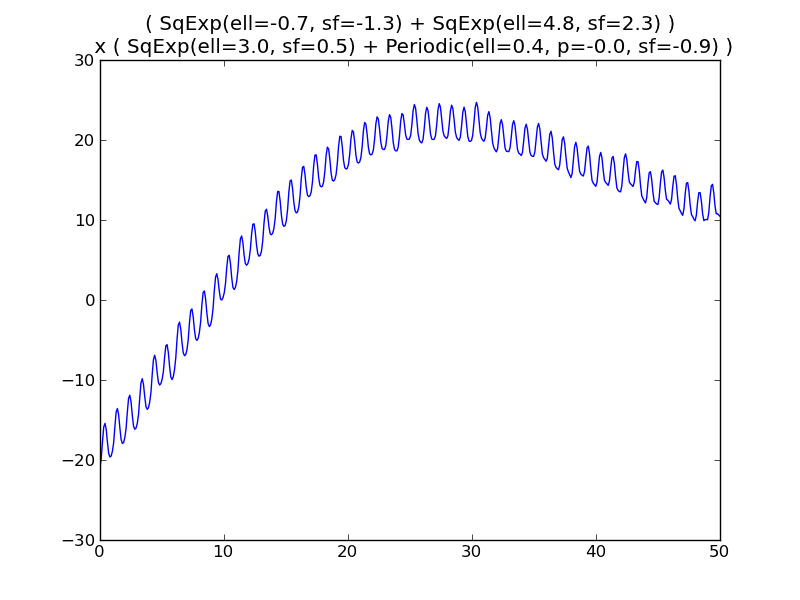
\includegraphics[width=\columnwidth]{../figures/mauna_prior_draw_best_cov_v3}
\caption{Another draw from our kernel.}
\end{figure}

\begin{figure}[h]
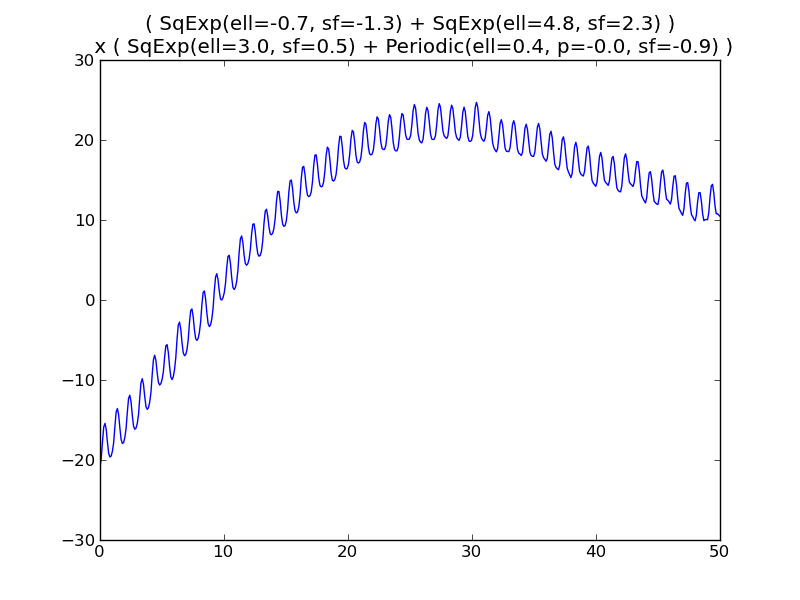
\includegraphics[width=\columnwidth]{../figures/mauna_prior_draw_best_cov_v3}
\caption{Another draw from our kernel.}
\end{figure}

\subsubsection{Load forecasting}

\subsection{Synthetic experiments}

\subsubsection{Bach Synthetic Dataset}
In addition to standard UCI repository datasets, we generated a synthetic dataset following the same recipe as \cite{DBLP:journals/corr/abs-0909-0844}: From a covariance matrix drawn from a Wishart distribution with 1024 degrees of freedom, we select 8 variables.  We then construct the non-linear function $f(X) = \sum_{i=1}^4 \sum_{j=1+1}^4 X_i X_j + \epsilon$, which sums all 2-way products of the first 4 variables, and adds Gaussian noise $\epsilon$.  This dataset is one which can be predicted well by a kernel which is a sum of two-way interactions over the first 4 variables, ignoring the extra 4 noisy copies.

This dataset was designed by \cite{DBLP:journals/corr/abs-0909-0844} to demonstrate the advantages of HKL over GP-ARD. 

 If the dataset is large enough, HKL can construct a hull around only those subsets of cross terms that are optimal for predicting the output.  GP-ARD, in contrast, can only learn to ignore the noisy copy variables, but cannot learn to ignore the higher-term interactions between the predictive variables.  However, a GP with an additive kernel can learn both to ignore irrelevant variables, and to ignore certain orders of interaction.  In this example, the additive GP is able to recover the relevant structure.

\subsection{Methods}

\subsubsection{Our method}
All of the experiments in this paper were performed using the standard GPML toolbox\footnote{Available at \texttt{http://www.gaussianprocess.org/gpml/code/}}; code to perform all experiments is available at the authors' website.

\subsubsection{Hierarchical Kernel Learning}
HKL\footnote{Code for HKL available at \texttt{http://www.di.ens.fr/\textasciitilde fbach/hkl/}} was run using the all-subsets kernel, which corresponds to the same set of kernels as considered by the additive GP with a squared-exp base kernel.



\section{DISCUSSION}

Machine learning can be more data-driven, analogous to the high-thoughput approaches being used in biology. 


\section{CONCLUSION}


\subsubsection*{Acknowledgements}


\bibliographystyle{format/icml2013}
\bibliography{gpss}

\end{document}
